\documentclass[twoside]{article}
\usepackage[a4paper]{geometry}
\geometry{verbose,tmargin=2.5cm,bmargin=2cm,lmargin=2cm,rmargin=2cm}
\usepackage{fancyhdr}
\pagestyle{fancy}

% nastavení pisma a~češtiny
\usepackage{lmodern}
\usepackage[T1]{fontenc}
\usepackage[utf8]{inputenc}
\usepackage[czech]{babel}

% odkazy
\usepackage{url}

\usepackage{float}
% vícesloupcové tabulky
\usepackage{multirow}
\usepackage{amssymb}
\usepackage{bbold}
\usepackage{amsmath}
\usepackage{mathtools}
\usepackage{commath}

% vnořené popisky obrázků
\usepackage{subcaption}

% automatická konverze EPS 
\usepackage{graphicx} 
\usepackage{epstopdf}
\epstopdfsetup{update}

\graphicspath{{./images}}

% odkazy a~záložky
\usepackage[unicode=true, bookmarks=true,bookmarksnumbered=true,
bookmarksopen=false, breaklinks=false,pdfborder={0 0 0},
pdfpagemode=UseNone,backref=false,colorlinks=true] {hyperref}

% Poznámky při překladu
\usepackage{xkeyval}	% Inline todonotes
\usepackage[textsize = footnotesize]{todonotes}
\presetkeys{todonotes}{inline}{}

%https://tex.stackexchange.com/questions/2783/bold-calligraphic-typeface
\DeclareMathAlphabet\mathbfcal{OMS}{cmsy}{b}{n}

% Zacni sekci slovem ukol
\renewcommand{\thesection}{Úkol \arabic{section}}
% enumerate zacina s pismenem
\renewcommand{\theenumi}{\alph{enumi}}

% smaz aktualni page layout
\fancyhf{}
% zahlavi
\usepackage{titling}
\fancyhf[HC]{\thetitle}
\fancyhf[HLE,HRO]{\theauthor}
\fancyhf[HRE,HLO]{\today}
 %zapati
\fancyhf[FLE,FRO]{\thepage}

% údaje o autorovi
\title{Automatické řízení: DÚ 5 -- Zpětná a~přímá vazba}
\author{Vojtěch Michal}
\date{\today}

\begin{document}

\maketitle

Obrázky se schématy systémů jsou v zadání dostupném na \cite{zadani}.

\section{Zpětná vazba}
Porovnejte dva systémy, jejichž schémata jsou na obrázcích v zadání.
Pro jednoznačnost označím horní systém písmenem A, dolní systém písmenem B.
Zjistěte, jaký mezi nimi může být rozdíl z hlediska stability. Rada: Najděte podmínky stability každého
z nich, porovnejte je a~případné rozdíly vysvětlete.

\textbf{Řešení:}
O stabilitě systému rozhoduje jeho charakteristický polynom. Nalezněme přenosy pro systém A
\begin{equation}
	G_A(s) = \frac{r(s)}{p(s)} \cdot \frac{\frac{b(s)}{a(s)} }{1 + \frac{b(s)}{a(s)} \cdot \frac{q(s)}{p(s)}} =
	\frac{r(s)}{p(s)} \cdot \frac{b(s) \cdot p(s)}{p(s) \cdot a(s) + b(s) \cdot q(s)}
\end{equation}
a pro systém B
\begin{equation}
	G_B(s) = r(s) \cdot \frac{\frac{b(s)}{a(s)} \cdot \frac{1}{p(s)}}{1 + \frac{b(s)}{a(s)} \cdot \frac{1}{p(s)} \cdot \frac{q(s)}{1}} =
	r(s) \cdot \frac{b(s) }{p(s) \cdot a(s) + b(s) \cdot q(s)}.
\end{equation}
Pakliže má být systém stabilní (studujeme vnitřní stabilitu, nikoli jen BIBO), poté musí být stabilní oba jeho subsystémy -- předfiltr
$\frac{r(s)}{p(s)}$ i~za ním kaskádně zapojená zpětnovazební smyčka. Na první pohled je vidět, že rozdíl systémů je v poloze
polynomu $p(s)$. V systému A se nalézá ve jmenovateli předfiltru, v systému B se nalézá ve jmenovateli přímé větve zpětnovazební
smyčky. Uzavření zpětné vazby (FB) vytváří v principu nový systém; pomocí FB je možné stabilizovat nestabilní soustavy.
Naopak seriové řazení systémů tuto vlastnost nemá. Jakmile je systém jednou nestabilní, není možné jej stabilizovat prostým 
seriovým připojením dalšího systému (krácení pólů povede na skryté módy, které budou vybuditelné například odlišnou konfigurací
počátečních podmínek).

Matematicky lze tuto myšlenku podložit analýzou charakteristických polynomů
\begin{equation}
	\begin{split}
		c_B(s) &= p(s) \cdot a(s) + b(s) \cdot q(s), \\
		c_A(s) &= p(s) \cdot (p(s) \cdot a(s) + b(s) \cdot q(s)) = p(s) \cdot c_B(s).
	\end{split}
\end{equation}
Pro stabilitu systému B je postačující, aby měly kořeny polynomu $c_B(s)$ zápornou reálnou část.
Pro stabilitu systému A je nezbytné totéž, nad to je ale ještě potřeba, aby samotné $p(s)$ bylo stabilní,
protože se nalézá ve jmenovateli samostatně.

\textbf{Závěr:} Uzavření zpětnovazební smyčky je schopno v jistém smyslu posunout kořeny polynomu $p(s)$
do stabilní oblasti. Jakmile však kolem systému FB uzavřen není, je nezbytné, aby byl sám o sobě stabilní.
Oba systémy budou mít z hlediska vnějšího modelu stejný přenos, protože $p(s)$ v čitateli a~jmenovateli přenosu $G_A(s)$
se proti sobě pokrátí, vnitřně však může nastat nestabilita a~signál na výstupu předfiltru $\frac{r(s)}{p(s)}$ poroste nade všechny meze.

\section{Přímá vazba}
Chování systému s přenosem $P(s) = P_1(s) P_2(s)$, kde
\begin{equation}
	P_1(s) = \frac{s+2}{s+1}, ~~~ P_2(s) = \frac{1}{s-1},
\end{equation}
ovlivňuje porucha $d(s)$, která přichází dovnitř soustavy dle obrázku v zadání.

Naštěstí tuto poruchu můžete před vstupem do soustavy měřit. Navrhněte přímovazební a
zpětnovazební část regulátoru (tedy přenosy $F(s)$ a~$C(s)$ dle obrázku) tak, aby porucha co nejméně
ovlivňovala výstup soustavy a~aby celý systém byl stabilní.
Rada: Nejprve vypočtete přenos poruchy na výstup soustavy. V tomto zvláštním případě lze tento přenos
velmi vhodně upravit jednoduchou volbou přímovazebního regulátoru. Potom navrhněte stabilizující
zpětnovazební regulátor. 

\textbf{Řešení:}
Odvoďme přenos z poruchy $d(s)$ na výstup systému $y(s)$ (pro lepší čitelnost vynechávám explicitní zmínky závislosti
přenosů $P_1$, $P_2$, $C$ a~$F$ a signálů $d$, $y_r$ a~$y$ na komplexní frekvenci $s$). Protože platí
\begin{equation}
	\begin{split}
		y = P_2 (d + P_1(C (-y) - F d)) &= P_2 d - P_2 P_1 C y - P_2 P_1 F d\\
		(1 + P_2 P_1 C)y &= P_2(1-P_1 F) d \\
		y &= \frac{P_2(1-P_1 F)}{1 + P_2 P_1 C} d,
	\end{split}
\end{equation}
je přenos z poruchy na výstup soustavy roven
\begin{equation}
	G_{dy}(s) = \frac{y(s)}{d(s)} = \frac{P_2(1-P_1 F)}{1 + P_2 P_1 C}.
	\label{eq:prenos}
\end{equation}

\subsection{Potlačení poruchy}
Pro maximální potlačení poruchy musí být přenos v rovnici \eqref{eq:prenos} nulový. Toho lze dosáhnout velkým jmenovatelem
($1 + P_2 P_1 C \rightarrow \infty$) a~nebo nulovým čitatelem. Nedává smysl snažit se vynulovat přenos soustavy $P_2(s)$,
musí tedy platit $ 1 - P_1 F = 0$, což nastane právě pro $F(s) = P_1^{-1} (s)$. Volbou
\begin{equation}
	F(s) = s - 1
\end{equation}
je proto zajištěno úplné potlačení přenosu poruchy $d(s)$ na výstup systému $y(s)$.

\begin{figure}[H]
	\centering
	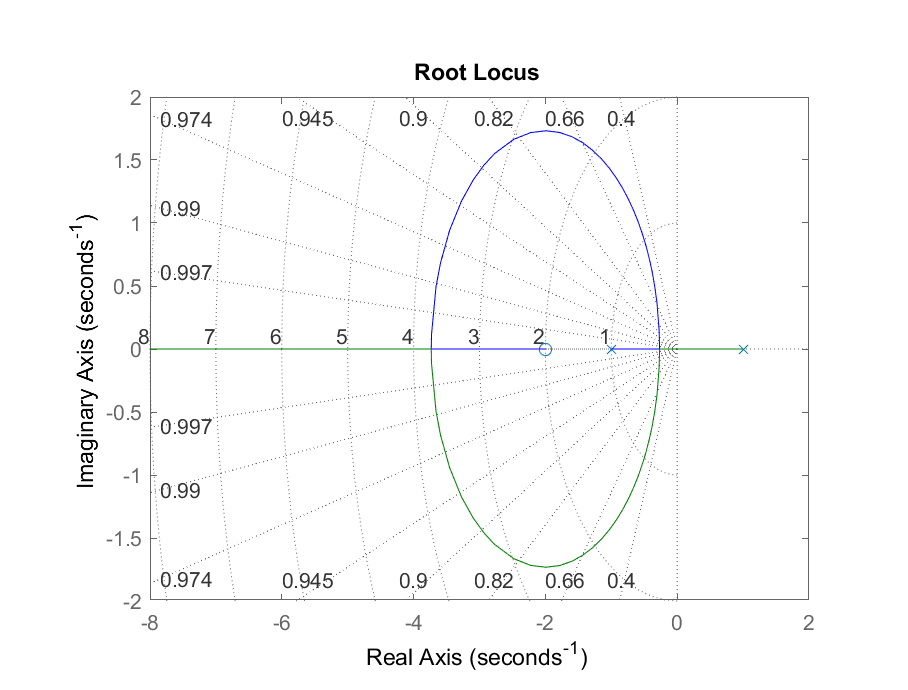
\includegraphics{rl.eps}
	\caption{Root locus pro přenos $P(s)$}
	\label{fig:rl}
\end{figure}

\subsection{Stabilita}
Pro zajištění stability je nezbytné, aby kořeny charakteristického polynomu měly reálné části záporné.
Póly přenosu z rovnice \eqref{eq:prenos} jsou takové hodnoty $s$, pro které platí $1 + P_2 P_1 C = 0$.
Jaký regulátor bychom mohli použít? Může nám pomoci root locus -- zpětnou vazbu uzavíráme kolem
soustavy $\frac{s+2}{s^2 - 1}$, ta má dva reálné póly a~jednu reálnou nulu. Podle jednoho z pravidel
bude procházet graf root locus po reálné ose na intervalech, které leží nalevo od lichého počtu pólů otevřené
zpětnovazební smyčky. Protože má soustava jeden pól v nestabilním bodě $s = 1$, musíme jej vhodným výběrem regulátoru $C(s)$ stáhnout
do stabilní levé poloroviny $s$. Na to stačí i~prostý proporcionální regulátor se zesílením $K \in \mathbb{R}$.
\begin{equation}
	\begin{split}
		1 + \underbrace{C(s)}_{K} \cdot \frac{s+2}{s+1} \frac{1}{s-1} &= 0 \\
		(s+1)(s-1) + K(s+2) &= 0 \\
		s^2 +K s +2K-1 &= 0. \\
	\end{split}
\end{equation}
Pro studium polohy pólů systému v závislosti na zesílení $K$ lze vykreslit root locus pro přenos $P(s)$ (viz obrázek~\ref{fig:rl}).
Pomocí nástroje \textit{rltool} v Matlabu lze určit, že nestabilní pól dosáhne průsečíku s imaginární osou
pro zesílení $K = 0.5$ a~pro libovolné větší $K$ již zůstane v otevřené levé polorovině $s$. Proto stabilitu systému zajistí libovolné $K > 0.5$.


\begin{thebibliography}{9}

	\bibitem{zadani} Zadání domácího úkolu \url{http://www.polyx.com/_ari/du/du_05.pdf}

\bibitem{motivace}
	Robert H. Bishop, Supplementary lectures to book \emph{Modern control systems, 13th edition} \url{https://www.youtube.com/watch?v=HanTvyEQI7U}

\end{thebibliography}












\end{document}

